\documentclass[12pt, titlepage]{article}

\usepackage{booktabs}
\usepackage{tabularx}
\usepackage{hyperref}
\hypersetup{
    colorlinks,
    citecolor=black,
    filecolor=black,
    linkcolor=red,
    urlcolor=blue
}
\usepackage[round]{natbib}
\usepackage{float}
\usepackage{geometry}
\usepackage{xcolor}
\usepackage{graphicx}
\usepackage{enumitem}

\usepackage{longtable}

%% Comments

\usepackage{color}

\newif\ifcomments\commentstrue %displays comments
\newif\ifcomments\commentsfalse %so that comments do not display

\ifcomments
\newcommand{\authornote}[3]{\textcolor{#1}{[#3 ---#2]}}
\newcommand{\todo}[1]{\textcolor{red}{[TODO: #1]}}
\else
\newcommand{\authornote}[3]{}
\newcommand{\todo}[1]{}
\fi

\newcommand{\wss}[1]{\authornote{blue}{SS}{#1}} 
\newcommand{\plt}[1]{\authornote{magenta}{TPLT}{#1}} %For explanation of the template
\newcommand{\an}[1]{\authornote{cyan}{Author}{#1}}

%% Common Parts

\newcommand{\progname}{Sayyara} % PUT YOUR PROGRAM NAME HERE
\newcommand{\authname}{Team 31
\\ SFWRENG 4G06
\\ Christopher Andrade
\\ Alyssa Tunney
\\ Kai Zhu
\\ Ethan Vince-Budan
\\ Collin Kan
\\ Harsh Gupta} % AUTHOR NAMES                  

\usepackage{hyperref}
    \hypersetup{colorlinks=true, linkcolor=blue, citecolor=blue, filecolor=blue,
                urlcolor=blue, unicode=false}
    \urlstyle{same}

\newcommand{\testpass}{\textcolor{green}{PASS}}
\newcommand{\testtbd}{\textcolor{orange}{TBD}}
\newcommand{\testfail}{\textcolor{red}{FAIL}}

\begin{document}

\title{Verification and Validation Report: \progname} 
\author{\authname}
\date{\today}
	
\maketitle

\pagenumbering{roman}

\section{Revision History}

\begin{tabularx}{\textwidth}{p{3cm}p{2cm}X}
\toprule {\bf Date} & {\bf Version} & {\bf Notes}\\
\midrule
March 3, 2023 & Rev 0 & Added testing results for NFRs\\
March 5, 2023 & Rev 0 & Added sections for Unit Testing and Automated Testing \\
March 8, 2023 & Rev 0 & Added testing reults for Look/Feel and Usability NFRs\\
\bottomrule
\end{tabularx}

~\newpage

\section{Symbols, Abbreviations and Acronyms}

\renewcommand{\arraystretch}{1.2}
\begin{tabularx}{\textwidth}{l X}
  \toprule		
  \textbf{symbol} & \textbf{description}\\
  \midrule 
  DDoS & Distributed Denial-of-service; when multiple systems flood the bandwidth or resources of a targeted system\\
  SessionID & A unique number that a web site's server assigns a signed in user for the duration of the user's visit\\
  CSRF Token & Unique, secret value generated server-side that is shared with the client. The client must include this CSRF token when submitting a form, etc.\\
  E2E & End-to-end \\
  \bottomrule
\end{tabularx}\\

\newpage

\tableofcontents

\listoftables %if appropriate

\listoffigures %if appropriate

\newpage

\pagenumbering{arabic}

\section{Introduction}

This document outlines the steps that have been taken to test and verify the requirements of the Sayyara application, and follow the general plans from the VnV Plan document. 

\section{Testing Methodology}

% Harsh
The web application architecture consists of a Django backend and NextJS frontend, deployed on Docker with an Nginx proxy routing the endpoints respectively. For backend unit testing, the pytest framework is utilized to write and execute unit tests for individual components or units of code in isolation. The code coverage of the unit tests is also tracked using the coverage.py.

For frontend unit testing as well as end-to-end testing, Playwright is used. This Node.js library provides a high-level API to interact with web browsers, simulating user interactions and verifying expected behavior. By combining backend unit testing with frontend unit and end-to-end testing, the entire system can be tested comprehensively, from the database to the user interface, helping to identify issues early in the development process and reduce the cost and time required for debugging and fixing issues later on.


\section{Functional Requirements Evaluation}
\subsection{Account Requirements}
\subsubsection{Registration}
\begin{enumerate}
    \item Id: FR-AR1-1\\
    Req: AuR1\\
    Description: registration of new account with valid account details\\
    Init State: \begin{itemize}[noitemsep,topsep=0pt]
        \item Empty account registration form is displayed.
        \item Username TestUser does not exist in account database.
    \end{itemize}
    Input: \begin{itemize}[noitemsep,topsep=0pt]
        \item username: TestUser
        \item password: somePassword
        \item first name: John
        \item last name: Doe
        \item email: sayyara.test@gmail.com
        \item phone: 5551234567
        \item role: customer
        \item click Submit button
    \end{itemize}
    Expected Output: Redirect to login page. New user exists in database with all fields matching input.\\
    Actual Output: \begin{itemize}[noitemsep,topsep=0pt]
        \item login view is displayed
        \item TestUser exists in account database
        \item TestUser.first\_name: John
        \item TestUser.last\_name: Doe
        \item TestUser.email: sayyara.test@gmail.com
        \item TestUser.phone: 555-123-4567
        \item role: customer
    \end{itemize}
    Pass/Fail: Passed

    \item Id: FR-AR1-2\\
    Req: AuR1\\
    Description: attempt registration of duplicate username\\
    Init State: \begin{itemize}[noitemsep,topsep=0pt]
        \item Empty account registration form is displayed.
        \item Username TestUser already exists in account database (details match input in test FR-AR1-1).
    \end{itemize}
    Input: \begin{itemize}[noitemsep,topsep=0pt]
        \item username: TestUser
        \item password: somePassword
        \item first name: John
        \item last name: Doe
        \item email: sayyara.test@gmail.com
        \item phone: 1112223333
        \item role: customer
        \item click Submit button
    \end{itemize}
    Expected Output: Stay on registration page, display duplicate username error, no change to account database.\\
    Actual Output: \begin{itemize}[noitemsep,topsep=0pt]
        \item no redirection occurred
        \item registration form displayed duplicate username error
        \item TestUser.phone: 555-123-4567
    \end{itemize}
    Pass/Fail: Passed

    \item Id: FR-AR1-3\\
    Req: AuR1\\
    Description: attempt registration using invalid password\\
    Init State: \begin{itemize}[noitemsep,topsep=0pt]
        \item Empty account registration form is displayed.
        \item Username TestUser does not exists in account database.
    \end{itemize}
    Input: \begin{itemize}[noitemsep,topsep=0pt]
        \item username: TestUser
        \item password: 123
        \item first name: John
        \item last name: Doe
        \item email: sayyara.test@gmail.com
        \item phone: 1112223333
        \item role: customer
        \item click Submit button
    \end{itemize}
    Expected Output: Stay on registration page, display password format error, no change to account database.\\
    Actual Output: \begin{itemize}[noitemsep,topsep=0pt]
        \item no redirection occurred
        \item registration form displayed invalid password format error
        \item TestUser does not exist in account database
    \end{itemize}
    Pass/Fail: Passed
    
\end{enumerate}

\subsubsection{Login}
\begin{enumerate}
    \item Id: FR-AR2-1\\
    Req: AuR2\\
    Description: login using valid password and password\\
    Init State: \begin{itemize}[noitemsep,topsep=0pt]
        \item Empty login form is displayed.
        \item Customer TestUser with password ``somePassword'' exists in database
    \end{itemize}
    Input: \begin{itemize}[noitemsep,topsep=0pt]
        \item username: TestUser
        \item password: somePassword
        \item click Login button
    \end{itemize}
    Expected Output: Receive access and refresh JWT tokens, redirect to homepage.\\ 
    Actual Output: \begin{itemize}[noitemsep,topsep=0pt]
        \item access token received in API fetch response
        \item refresh token received in API fetch response
        \item homepage is displayed with greeting message for TestUser
    \end{itemize}
    Pass/Fail: Passed

    \item Id: FR-AR2-2A\\
    Req: AuR2\\
    Description: attempt login using the wrong password\\
    Init State: \begin{itemize}[noitemsep,topsep=0pt]
        \item Empty login form is displayed.
        \item Customer TestUser with password ``somePassword'' exists in database
    \end{itemize}
    Input: \begin{itemize}[noitemsep,topsep=0pt]
        \item username: TestUser
        \item password: wrongPassword
        \item click Login button
    \end{itemize}
    Expected Output: Stay on login page, display invalid username/password error.\\ 
    Actual Output: \begin{itemize}[noitemsep,topsep=0pt]
        \item no redirection occurred
        \item login form displays username/password error
        \item no token received in API response
    \end{itemize}
    Pass/Fail: Passed

    \item Id: FR-AR2-2B\\
    Req: AuR2\\
    Description: attempt login to non-existent user\\
    Init State: \begin{itemize}[noitemsep,topsep=0pt]
        \item Empty login form is displayed.
        \item TestUser does not exists in account database
    \end{itemize}
    Input: \begin{itemize}[noitemsep,topsep=0pt]
        \item username: TestUser
        \item password: somePassword
        \item click Login button
    \end{itemize}
    Expected Output: Stay on login page, display invalid username/password error.\\ 
    Actual Output: \begin{itemize}[noitemsep,topsep=0pt]
        \item no redirection occurred
        \item login form displays username/password error
        \item no token received in API response
    \end{itemize}
    Pass/Fail: Passed

    \item Id: FR-AR2-3\\
    Req: AuR3\\
    Description: unauthorized attempt to change password\\
    Init State: \begin{itemize}[noitemsep,topsep=0pt]
        \item TestUser with password ``somePassword'' exists in account database
        \item command prompt initialized
    \end{itemize}
    Input: CURL --request POST --url http://localhost/api/auth/users/set\_password/ --header `Content-Type: application/json' --data `{
	``current\_password'':``password'',
	``new\_password'':``newPassword''}'
    Expected Output: 401 unauthorized error.\\ 
    Actual Output: \begin{itemize}[noitemsep,topsep=0pt]
        \item 401 Unauthorized error
    \end{itemize}
    Pass/Fail: Passed
\end{enumerate}

\subsubsection{User Profile}
\begin{enumerate}
    \item Id: FR-PAR3-1\\
    Req: PAR3\\
    Description: Editting user profile\\
    Init State: \begin{itemize}[noitemsep,topsep=0pt]
        \item Profile page is displayed
        \item Customer TestUser exists in database
        \item Logged in as TestUser
    \end{itemize}
    Input: \begin{itemize}[noitemsep,topsep=0pt]
        \item click Edit button
        \item last name: Dow
        \item phone: 555-123-4444
        \item click Update button
    \end{itemize}
    Expected Output: Profile page displays updated information\\ 
    Actual Output: \begin{itemize}[noitemsep,topsep=0pt]
        \item last name: Dow
        \item phone: 555-123-4444
        \item all other fields: unchanged
    \end{itemize}
    Pass/Fail: Passed

    \item Id: FR-PAR3-2\\
    Req: PAR3\\
    Description: Editting user profile with invalid details\\
    Init State: \begin{itemize}[noitemsep,topsep=0pt]
        \item Profile page is displayed
        \item Customer TestUser exists in database
        \item Logged in as TestUser
    \end{itemize}
    Input: \begin{itemize}[noitemsep,topsep=0pt]
        \item click Edit button
        \item first name: $<$blank$>$
        \item phone: 555
        \item click Update button
    \end{itemize}
    Expected Output: Profile page stays in edit mode, displays invalid form fields error\\ 
    Actual Output: \begin{itemize}[noitemsep,topsep=0pt]
        \item silently failed. No error was displayed
        \item profile page exited edit mode
        \item TestUser profile is unchanged
    \end{itemize}
    Pass/Fail: Failed
\end{enumerate}

    \subsection{Quote Requirements}

        \subsubsection{Summary of Test Cases}
            \begin{table}[H]
                \centering
                \begin{tabularx}{\textwidth}{|l|p{2.3cm}|X|X|c|}
                    \hline
                    Id & Reference Requirement & Summary & Expected Output & Pass/Fail \\ \hline
                    \hyperref[FR-QR1-1.1]{FR-QR1-1.1} & QR1 & Vehicle owner sends a message on quote request & Message visible for both vehicle owner and shop owner/employees & \testpass \\ \hline
                    \hyperref[FR-QR1-1.2]{FR-QR1-1.2} & QR1 & Shop owner sends a message on quote request & Message visible for both vehicle owner and shop owner/employee & \testpass \\ \hline
                    \hyperref[FR-QR2-1.1]{FR-QR2-1.1} & QR2, QR3 & User selects the ``New Quote Request'' button & Modal for setting up a new quote is displayed & \testpass \\ \hline
                    \hyperref[FR-QR2-1.2]{FR-QR2-1.2} & QR2, QR3 & User fills in quote request form with \textit{correct/valid} data and submits the form & A new quote request is created, stored and becomes viewable by selected shops & \testpass \\ \hline
                    \hyperref[FR-QR2-1.3]{FR-QR2-1.3} & QR2, QR3 & User fills in quote request form with \textit{incorrect/invalid} data and attempts to submit the form & User is shown an error message indicating which part(s) of their input are invalid & \testpass \\ \hline
                \end{tabularx}
                \caption{Summary of tests for functional requirements from section 10.1.6 of the SRS}
            \end{table}

        \subsubsection{Individual Test Cases}
            \begin{enumerate}
                \item \textbf{FR-QR1-1.1} \label{FR-QR1-1.1} \\ Requirements: QR1 \\
                    Description: Vehicle owner sending a message on a quote request \\
                    Initial State/Setup: \begin{itemize}
                        \item Authenticated as vehicle owner
                        \item Quote request successfully created
                    \end{itemize}
                    Input: \begin{itemize}
                        \item Expand quote request and select shop from list of pending responses
                        \item Enter message ``Test Message''
                        \item Press ``Submit reply'' button
                    \end{itemize}
                    Expected output: Message saved to quote request conversation, message visible to both vehicle owner and shop owner/employees \\
                    Actual output: \begin{itemize}
                        \item Vehicle owner's view updates to display new message
                        \item Shop owner/employee's view automatically refreshes in order to display new message
                    \end{itemize}
                    Result: \testpass

                \item \textbf{FR-QR1-1.2} \label{FR-QR1-1.2} \\ Requirements: QR1 \\
                    Description: Shop owner sending a message on a quote request \\
                    Initial State/Setup: \begin{itemize}
                        \item Authenticated as shop owner
                        \item Quote request created and sent to owner's shop
                    \end{itemize}
                    Input: \begin{itemize}
                        \item Select quote from list
                        \item Enter message ``Test Reply''
                        \item Press ``Submit reply'' button
                    \end{itemize}
                    Expected output: Message saved to quote request conversation, message visible to both vehicle owner and shop owner/employees \\
                    Actual output: \begin{itemize}
                        \item Shop owner's view updates to display new message
                        \item Vehicle owner's view automatically refreshes in order to display new message
                    \end{itemize}
                    Result: \testpass
                    
                \item \textbf{FR-QR2-1.1} \label{FR-QR2-1.1} \\ Requirements: QR2, QR3 \\
                    Description: Accessing quote adding functionality \\
                    Initial State/Setup: \begin{itemize}
                        \item Authenticated as vehicle owner
                        \item Navigate to the Quotes page
                    \end{itemize}
                    Input: \begin{itemize}
                        \item Select the ``New Quote Request'' button
                    \end{itemize}
                    Expected output: Modal for setting up a new quote is displayed \\
                    Actual output: Modal for setting up a new quote is displayed \\
                    Result: \testpass

                \item \textbf{FR-QR2-1.2} \label{FR-QR2-1.2} \\ Requirements: QR2, QR3 \\
                    Description: Creating a quote request (normal input) \\
                    Initial State/Setup: \begin{itemize}
                        \item Authenticated as vehicle owner
                        \item Account has at least 1 associated vehicle
                        \item Navigate to the Quotes page
                        \item Select the ``New Quote Request'' button
                    \end{itemize}
                    Input: \begin{itemize}
                        \item Vehicle for servicing: 1st option in list (vehicle associated with account)
                        \item Description: ``Normal Description''
                        \item Additional photo information: N/A (\textbf{TODO})
                        \item Part preference: New
                        \item Available shops: Every option selected
                        \item Availability: ``Monday 12:00 - 15:00''
                        \item Click ``Submit quote request'' button
                    \end{itemize}
                    Expected output: \begin{itemize}
                        \item New quote request matching the given information is created
                        \item New quote is now visible on the Quotes page
                        \item Modal is automatically closed to prevent re-submission
                    \end{itemize}
                    Actual output: \begin{itemize}
                        \item Modal is automatically closed
                        \item Quote appears in list for customer
                        \item Quote appears in list for shop owners \& employees
                    \end{itemize}
                    Result: \testpass

                \item \textbf{FR-QR2-1.3} \label{FR-QR2-1.3} \\ Requirements: QR2, QR3  \\
                    Description: Creating a quote request (abnormal input) \\
                    Initial State/Setup: See \hyperref[FR-QR2-1.2]{FR-QR2-1.2} \\
                    Input: \begin{itemize}
                        \item Vehicle for servicing: 1st option in list (vehicle associated with account)
                        \item Description: ``Abnormal Description''
                        \item Additional photo information: N/A (\textbf{TODO})
                        \item Part preference: Used
                        \item Available shops: None selected
                        \item Availability: `` '' (Empty string)
                        \item Click ``Submit quote request'' button
                    \end{itemize}
                    Expected output: Quote request creation fails, user is notified, modal remains open \\
                    Actual output: \begin{itemize}
                        \item Modal window remains open
                        \item No new quote request is created
                        \item Message displayed to user indicating the location \& type of error
                    \end{itemize}
                    Result \testpass
            \end{enumerate}
    

    \subsection{Vehicle Requirements}
        \subsubsection{Summary of Test Cases}
            \begin{table}[H]
                \centering
                \begin{tabularx}{\textwidth}{|l|p{2.3cm}|X|X|c|}
                    \hline
                    Id & Reference Requirement & Summary & Expected Output & Pass/Fail \\ \hline
                    \hyperref[FR-VE1-1.1]{FR-VE1-1.1} & PAR5 & User selects the ``New Vehicle'' button & Modal for creating a new vehicle is displayed & \testpass \\ \hline
                    \hyperref[FR-VE1-1.2]{FR-VE1-1.2} & PAR5 & User adds a vehicle to their account & New vehicle is created and linked to user & \testpass \\ \hline
                    \hyperref[FR-VE1-1.3]{FR-VE1-1.3} & PAR5 & User removes a vehicle from their account (normal case) & Vehicle deleted and no longer visible on profile & \testfail \\ \hline
                    \hyperref[FR-VE1-1.4]{FR-VE1-1.4} & PAR5 & User removes a vehicle from their account (abnormal case) & Error message is displayed, and vehicle remains & \testfail \\ \hline
                \end{tabularx}
                \caption{Summary of test cases for Vehicles module}
            \end{table}

        \subsubsection{Individual Test Cases}
            \begin{enumerate}
                \item \textbf{FR-VE1-1.1} \label{FR-VE1-1.1} \\ Requirements: PAR5 \\
                    Description: User selects the ``New Vehicle'' button \\
                    Initial State/Setup: \begin{itemize}
                        \item Authenticated as Vehicle owner
                        \item Profile page is selected
                        \item No prior vehicles added to account
                    \end{itemize}
                    Input: \begin{itemize}
                        \item Click ``Add vehicle'' button
                    \end{itemize}
                    Expected output: Modal for creating a new vehicle is displayed \\
                    Actual output: Modal for creating a new vehicle is displayed \\
                    Result: \testpass
                    
                \item \textbf{FR-VE1-1.2} \label{FR-VE1-1.2} \\ Requirements: PAR5 \\
                    Description: User adds a new vehicle to their account \\
                    Initial State/Setup: \begin{itemize}
                        \item Authenticated as vehicle owner
                        \item Profile page is selected
                    \end{itemize}
                    Input: \begin{itemize}
                        \item Click ``Add vehicle'' button
                        \item Make: Toyota
                        \item Model: Corolla
                        \item Year: 2009
                        \item Plate number: ``ABC 123''
                        \item VIN: ``2HSABC3489AIBF76H''
                        \item Click ``Submit'' button
                    \end{itemize}
                    Expected output: \begin{itemize}
                        \item Add vehicle modal is automatically closed to avoid re-submission
                        \item Vehicle with matching information is added to user account
                        \item Vehicle is visible on profile page
                    \end{itemize}
                    Actual output: \begin{itemize}
                        \item Vehicle modal is closed automatically
                        \item Page must be manually refreshed in order for new vehicle to appear on profile
                    \end{itemize}
                    Result: \testpass

                \item \textbf{FR-VE1-1.3} \label{FR-VE1-1.3} \\ Requirements: PAR5 \\
                    Description: User removes a vehicle from their account (normal case) \\
                    Initial state/setup: \begin{itemize}
                        \item Authenticated as vehicle owner
                        \item At least one vehicle created and associated with current account
                        \item That vehicle must \textit{not} be associated with any quote requests/quotes
                        \item Profile page is selected
                    \end{itemize}
                    Input: \begin{itemize}
                        \item Click ``Remove Vehicle'' Button on vehicle component
                    \end{itemize}
                    Expected output: Vehicle is removed from user account, and is no longer visible from profile page
                    Actual output: No method to delete vehicles is currently present on the profile page \\
                    Result: \testfail

                \item \textbf{FR-VE1-1.4} \label{FR-VE1-1.4} \\ Requirements: PAR5 \\
                    Description: User attempts to remove a vehicle from their account, which is attached to at least one quote request, quote or appointment \\
                    Initial state/setup: \begin{itemize}
                        \item Authenticated as vehicle owner
                        \item One vehicle created and associated with current account
                        \item At least one quote request created using current user's vehicle
                        \item Profile page is selected
                    \end{itemize}
                    Input: \begin{itemize}
                        \item Click ``Remove Vehicle'' button on vehicle component
                    \end{itemize}
                    Expected output: \begin{itemize}
                        \item Error message is displayed explaining to user why vehicle could not be removed
                        \item Vehicle remains attached to user account
                    \end{itemize}
                    Actual output: No method to delete vehicles is currently present on the profile page \\
                    Result: \testfail
            \end{enumerate}
            
            
        \subsection{Appointment Requirements}
            \subsubsection{Summary of Test Cases}
            \begin{table}[H]
                \centering
                \begin{tabularx}{\textwidth}{|l|p{2cm}|X|X|c|}
                    \hline
                    Id & Reference Requirement & Summary & Expected Output & Pass/Fail \\ \hline
                    \hyperref[FR-AP1-1.1]{FR-AP1-1.1} & APR1 &  Shop owners should be able to change their shop's availability settings for appointments on the calendar. & The shop owner should be able to successfully change the availability settings for appointments. & \testpass \\ \hline
                    \hyperref[FR-AP2-1.1]{FR-AP2-1.1} & APR2 &  All types of users should be able to schedule appointments to service a vehicle. & The user should be able to successfully schedule an appointment to service a vehicle. & \testpass \\ \hline
                    % \hyperref[FR-AP3-1.1]{FR-AP3-1.1} & APR3 & Customers should only be able to schedule appointments if a quote has been received and approved by a shop, or if the job is pre-approved that does not require special information and pricing. & Appointments should only be able to be scheduled if the conditions in the requirement have been met. & \testpass \\ \hline
                    \hyperref[FR-AP4-1.1]{FR-AP4-1.1} & APR4 & All users should be able to optionally include a note in the appointment booking for organizational purposes. & The user should be able to add a note to the appointment booking. & \testpass \\ \hline
                    \hyperref[FR-AP5-1.1]{FR-AP5-1.1} & APR5 & Customers should be able to interact with a virtual AI assistant to assist the user in scheduling an appointment. & The AI assistant should be able to help the user schedule an appointment. & \testfail \\ \hline
                \end{tabularx}
                \caption{Test Cases}
                \label{tab:Test_Cases}
            \end{table}
            
        \subsubsection{Individual Test Cases}
            \begin{enumerate}
                \item \textbf{FR-AP1-1.1} \label{FR-AP1-1.1} \\ Requirements: APR1 \\
                    Description: Test that shop owners can change their shop's availability settings for appointments on the calendar. \\
                    Initial State/Setup: \begin{itemize}
                        \item Shop owner is logged into their account
                    \end{itemize}
                    Input: \begin{itemize}
                        \item Shop owner changes the availability settings for the day
                        \item Inputs:
                            \begin{itemize}
                                \item Quote
                                \item Title
                                \item Description
                                \item Time Estimate
                                \item Price Estimate
                                \item Message
                                \item Reservation
                            \end{itemize}
                    \end{itemize}
                    Expected output: The shop owner should be able to successfully change the availability settings for appointments. \\
                    Actual output: The shop owner is able to successfully change the availability settings for appointments. \\
                    Result: \testpass
                    
                    
                \item \textbf{FR-AP2-1.1} \label{FR-AP2-1.1} \\ Requirements: APR2 \\
                    Description: Test that shops can schedule appointments to service a vehicle. \\
                    Initial State/Setup: \begin{itemize}
                        \item User is logged into their account
                    \end{itemize}
                    Input: \begin{itemize}
                        % \item User select a service for their vehicle
                        \item User selects an available appointment time
                    \end{itemize}
                    Expected output: The user should be able to successfully schedule an appointment to service a vehicle. \\
                    Actual output: The user is able to successfully schedule an appointment to service a vehicle. \\
                    Result: \testpass 
                    
                    
                % \item \textbf{FR-AP3-1.1} \label{FR-AP3-1.1} \\ Requirements: APR3 \\
                %     Description: Test that customers can only schedule appointments if a quote has been received and approved by a shop, or if the job is pre-approved that does not require special information and pricing. \\
                %     Initial State/Setup: \begin{itemize}
                %         \item Quote is either pre-approved or approved by the shop
                %         \item User is logged into their account
                %     \end{itemize}
                %     Input: \begin{itemize}
                %         \item User select a service for their vehicle
                %         \item User selects an available appointment time
                %     \end{itemize}
                %     Expected output: Appointments should only be able to be scheduled if the conditions in the requirement have been met. \\
                %     Actual output: Appointments are only able to be scheduled if the conditions in the requirement have been met. \\
                %     Result: \testpass
                    
                    
                \item \textbf{FR-AP4-1.1} \label{FR-AP4-1.1} \\ Requirements: APR4 \\
                    Description: Test that all users can optionally include a note in the appointment booking for organizational purposes. \\
                    Initial State/Setup: \begin{itemize}
                        \item User is logged into their account
                        \item User selects an available appointment time
                    \end{itemize}
                    Input: \begin{itemize}
                        \item User adds a note to the appointment booking
                        \item Inputs: \begin{itemize}
                            \item Appointment
                            \item Note
                        \end{itemize}
                    \end{itemize}
                    Expected output: The user should be able to add a note to the appointment booking. \\
                    Actual output: The user is able to add a note to the appointment booking. \\
                    Result: \testpass
                    
                    
                \item \textbf{FR-AP5-1.1} \label{FR-AP5-1.1} \\ Requirements: APR5 \\
                    Description: Test that customers can interact with a virtual AI assistant to assist the user in scheduling an appointment. \\
                    Initial State/Setup: \begin{itemize}
                        \item User is logged into their account
                    \end{itemize}
                    Input: \begin{itemize}
                        \item User interacts with the AI assistant to schedule an appointment
                    \end{itemize}
                    Expected output: The AI assistant should be able to help the user schedule an appointment. \\
                    Actual output: Fails with NotImplemented Error \\
                    Result: \testfail
                    \end{enumerate}

        \subsection{Shop Lookup Requirements}
            \subsubsection{Summary of Test Cases}
            \begin{table}[H]
                \centering
                \begin{tabularx}{\textwidth}{|l|p{2cm}|X|X|c|}
                    \hline
                    Id & Reference Requirement & Summary & Expected Output & Pass/Fail \\ \hline
                    \hyperref[FR-SL-1.1]{FR-SL1-1.1} & SL1 & Customers should be able to search for shops by name. & \testpass \\ \hline
                    \hyperref[FR-SL-2.1]{FR-SL2-1.1} & SL2 & Customers should be able to search for shops by address, postal code, city, country, etc. & \testpass \\ \hline
                    \hyperref[FR-SL-3.1]{FR-SL3-1.1} & SL3 & The system should be able to return a set of coordinates (geolocation) if given a valid address. & \testpass \\ \hline
                    \hyperref[FR-SL-4.1]{FR-SL4-1.1} & SL4 & Customers should be able to filter out shops that they think are too far from thei current location or a speficied address. & \testpass \\ \hline
                    \hyperref[FR-SL-5.1]{FR-SL5-1.1} & SL5 & Customers should be able filter out shop that do not provide the service or services that they are looking for. & \testfail \\ \hline
                    \hyperref[FR-SL-5.1]{FR-SL6-1.1} & SL6 & Customers should be able to sort the search results alphabetically & \testfail \\ \hline
                    \hyperref[FR-SL-5.1]{FR-SL7-1.1} & SL7 & Customers should be able to sort the search results from closest to furthest (or vice versa) & \testfail \\ \hline
                \end{tabularx}
                \caption{Test Cases}
                \label{tab:Test_Cases}
            \end{table}
            
        \subsubsection{Individual Test Cases}
            \begin{enumerate}
                \item \textbf{FR-SL1.1} \label{FR-SL1.1} \\ Requirements: SL1 \\
                    Description: Test that customers search shop by name. \\
                    Initial State/Setup: Customer account is logged in, there are multiple shops in the database. \\
                    Input: Search query
                    Expected output: List of shops containing the string\\
                    Actual output: Sorted list (alphabetically)\\
                    Result: \testpass
                    
                    
                \item \textbf{FR-SL2.1} \label{FR-SL2.1} \\ Requirements: SL2 \\
                    Description: Test that customers can sort search results by name. \\
                    Initial State/Setup: Customer account is logged in, there are multiple shops in the database. \\
                    Input: Boolean
                    Expected output. Sorted list (alphabetically)\\
                    Actual output: Sorted list (alphabetically)\\
                    Result: \testpass
                    
                    
                \item \textbf{FR-SL3.1} \label{FR-SL3.1} \\ Requirements: SL3 \\
                    Description: Test that customers can sort search results by name. \\
                    Initial State/Setup: Customer account is logged in, there are multiple shops in the database. \\
                    Input: Boolean
                    Expected output. Sorted list (alphabetically)\\
                    Actual output: Sorted list (alphabetically)\\
                    Result: \testpass
                    
                    
                \item \textbf{FR-SL4.1} \label{FR-SL4.1} \\ Requirements: SL4 \\
                    Description: Test that customers can sort search results by name. \\
                    Initial State/Setup: Customer account is logged in, there are multiple shops in the database. \\
                    Input: Boolean
                    Expected output. Sorted list (alphabetically)\\
                    Actual output: Sorted list (alphabetically)\\
                    Result: \testpass
                    
                    
                \item \textbf{FR-SL5.1} \label{FR-SL5.1} \\ Requirements: SL5 \\
                    Description: Test that customers can sort search results by name. \\
                    Initial State/Setup: Customer account is logged in, there are multiple shops in the database. \\
                    Input: Boolean
                    Expected output. Sorted list (alphabetically)\\
                    Actual output: Sorted list (alphabetically)\\
                    Result: \testpass

                \item \textbf{FR-SL6.1} \label{FR-SL6.1} \\ Requirements: SL6 \\
                    Description: Test that customers can sort search results by name. \\
                    Initial State/Setup: Customer account is logged in, there are multiple shops in the database. \\
                    Input: Boolean
                    Expected output. Sorted list (alphabetically)\\
                    Actual output: Sorted list (alphabetically)\\
                    Result: \testpass

                \item \textbf{FR-SL7.1} \label{FR-SL7.1} \\ Requirements: SL7 \\
                    Description: Test that customers can sort search results by distance. \\
                    Initial State/Setup: Customer account is logged in, there are multiple shops in the database. \\
                    Input: Boolean
                    Expected output. Sorted list (by distance)\\
                    Actual output: Sorted list (by distance)\\
                    Result: \testpass
                    \end{enumerate}

                    
\newpage

\section{Nonfunctional Requirements Evaluation}

\subsection{Look and Feel}

    \begin{longtable}{|p{0.1\textwidth}|p{0.1\textwidth}|p{0.2\textwidth}|p{0.15\textwidth}|p{0.1\textwidth}|p{0.1\textwidth}|p{0.1\textwidth}|}
        \hline
        
        Test ID & Req & Desc & Input & Act. Result & Exp. Result & Pass/Fail \\
        \hline
        
        NFR-LFR1-1 &
        LFR1 & 
        Looping through all web components that are of the type "NextPage", and checking that no more than 5 "NextPage" web components are rendered inside as children components to avoid overly deep/confusing, interaction levels, with this test outputting the maximum depth found & 
        All "NextPage" web components &
        3 &
        \textless = 5 &
        Pass \\
        \hline

        NFR-LFR2-1 &
        LFR2 & 
        Looping through all HTML elements that are rendered in the absolute position (relative to the nearest positioned component; moves along with page scrolling), and checking that each contains a "box-shadow" CSS style &
        All absolutely positioned HTML elements &
        true &
        true &
        Pass \\
        \hline

        NFR-LFR3-1 &
        LFR3 & 
        Looping through all HTML elements with a class name containing a "panel-" prefix, indicating it is a panel whose visibility can be toggled, and checking if they contain a "transform" CSS property for smooth transitions &
        All HTML elements with "panel-" styling class prefix &
        true (no elements found) &
        true &
        Pass \\
        \hline

        NFR-LFR4-1 &
        LFR4 & 
        Looping through all HTML elements with a "border" style and checking if they also contain a "border-radius" style for smoothed edges &
        All HTML elements with a "border" style &
        true &
        true &
        Pass \\
        \hline

        NFR-LFR5-1 &
        LFR5 & 
        Looping through all HTML elements with a "color" style and checking if the corresponding hex code is in a predefined colour palette &
        All HTML elements with a "color" style &
        true &
        true &
        Pass \\
        \hline
    \caption{Look and Feel Tests and Results}
    \end{longtable}

\subsection{Usability}

\begin{longtable}{|p{0.1\textwidth}|p{0.1\textwidth}|p{0.2\textwidth}|p{0.15\textwidth}|p{0.1\textwidth}|p{0.1\textwidth}|p{0.1\textwidth}|}
        \hline
        
        Test ID & Req & Desc & Input & Act. Result & Exp. Result & Pass/Fail \\
        \hline
        
        NFR-UHR1-1 &
        UHR1 & 
        A user who has little technical background is asked to perform the common actions of the customer workflow and to rate the easiness of using the UI from 1-10 & 
        N/A &
        9 &
        \textgreater = 8 &
        Pass \\
        \hline

        NFR-UHR1-2 &
        UHR1 & 
        A user who has little technical background is asked to perform the common actions of the shop owner/employee workflow and to rate the easiness of using the UI from 1-10 & 
        N/A &
        8 &
        \textgreater = 8 &
        Pass \\
        \hline

        NFR-UHR2-1 &
        UHR2 & 
        Query all interactable HTML elements and make sure they have accessibility support through "index" and "role" tags as well as keyboard listeners & 
        Interactable HTML elements (such as buttons) &
        false (still requiring full implementation, only working in some parts of app) &
        true  &
        Fail \\
        \hline

        NFR-UHR3-1 &
        UHR3 & 
        A user who has little technical background is asked to guess how many interactable components there are, given different pages of the website, and is tested to see if \textgreater = 80 percent accuracy is achieved overall &
        Various pages of the application &
        90 percent &
        \textgreater = 80 percent &
        Pass \\
        \hline

        NFR-UHR4-1 &
        UHR4 & 
        Query all interactable HTML elements and make sure they do not have any double click event handlers & 
        Interactable HTML elements (such as buttons) &
        true &
        true  &
        Pass \\
        \hline

        NFR-UHR5-1 &
        UHR5 & 
        Query all HTML "input" tag elements (without a selectable list) and make sure they are tagged as search bars, for authentication/profile, or for chatting purposes &
        All "input" tag HTML elements without a dropdown list &
        true &
        true  &
        Pass \\
        \hline
    \caption{Usability Tests and Results}
    \end{longtable}

		
\subsection{Performance}
\subsubsection{System Uptime}
References requirement NFR-PR1-1 \\

% \noindent As of writing this report, the team is currently in the process of setting up the application so that it is deployed and hosted such that it can be accessed by anyone. Once this is completed, stress testing through the use of a tool such as JMeter that can send several responses from simulated users to the system in attempts to overwhelm it will be performed. This tool simulates a DDoS attack and the team's goal is to ensure that something like this would not crash the web server if it were to occur once deployment is completed.

As of revision 1, the application does not need to be deployed as per our project supervisor Nabil. System uptime testing will not be required for this revision.

\subsubsection{System Storage Usage}
References requirement NFR-PR2-1\\

This testing is done to ensure the browser is not storing any unnecessary information and is not storing any information that could lead to harmful behaviour by external users.

\begin{table}[H]
    \centering
    \begin{tabularx}{\textwidth}{|c|p{2.3cm}|p{2.4cm}|p{2.5cm}|p{2.2cm}|p{2cm}|}
        \hline
        Id & Reference Requirement & User Action & Expected Output & Actual Output & Pass/Fail\\ \hline
        SSU-1 & NFR-PR2-1 & User registers an account, signs in, fills in forms on the website, and utilizes search functions & User login info, SessionID, CSRF token saved & The only information saved on the user's browser is their basic login information, their SessionID, and the CSRF token & \textcolor{green}{Pass} \\ \hline
    \end{tabularx}
    \caption{System storage usage test}
    %\label{tab:my_label}
\end{table}

\begin{figure}[H]
    \centering
    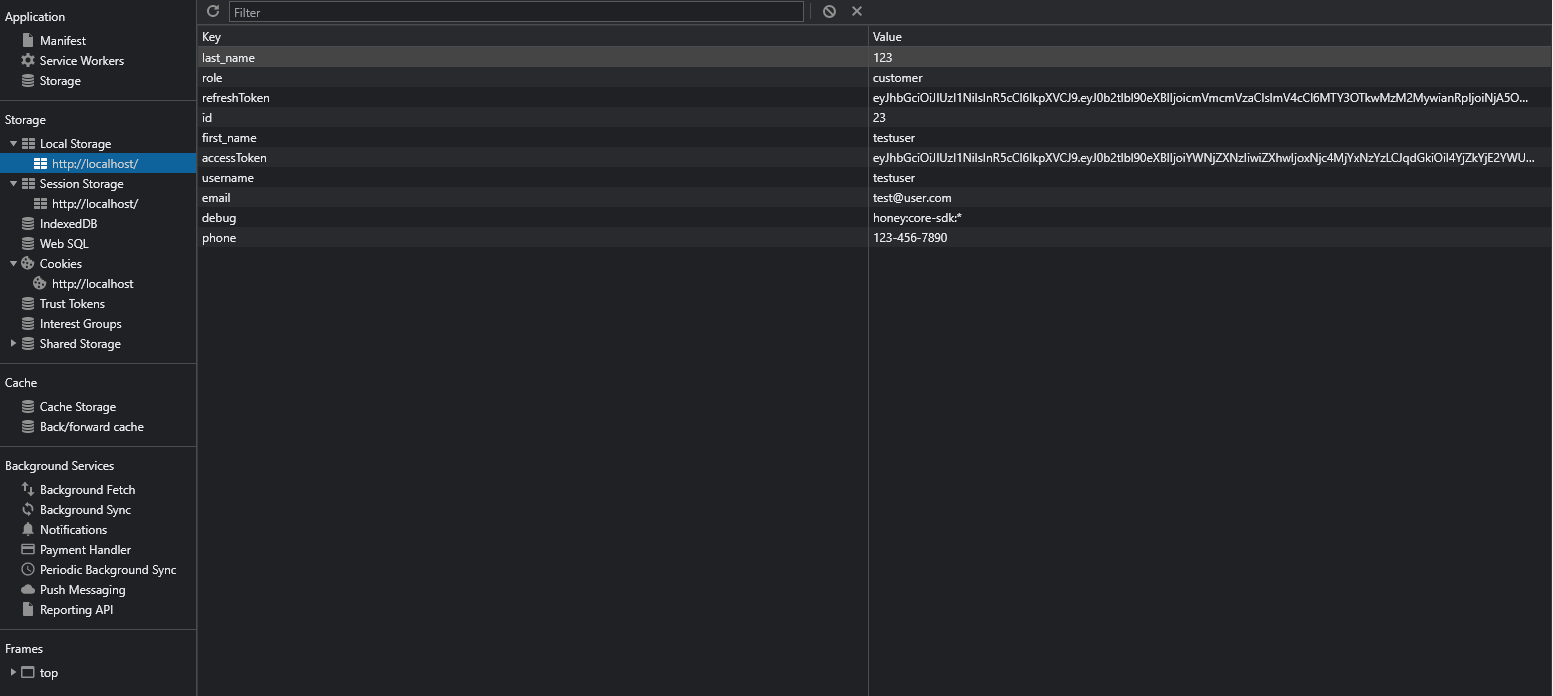
\includegraphics[width=\textwidth]{VnVReport/result_images/ssu_storage.png}
    \caption{Storage containing information from logged in user}
    \label{fig:ssu_storage}
\end{figure}

\begin{figure}[H]
    \centering
    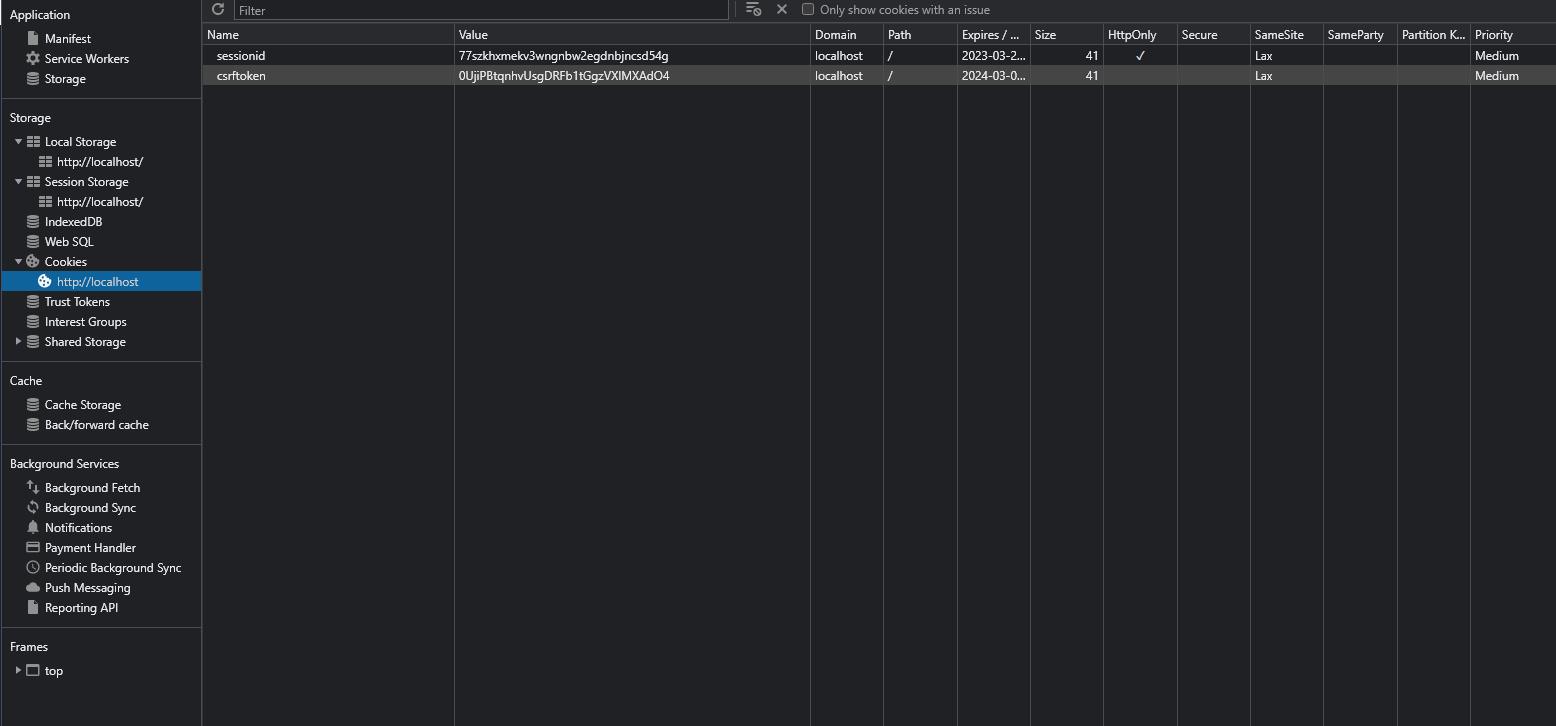
\includegraphics[width=\textwidth]{VnVReport/result_images/ssu_cookies.png}
    \caption{Storage containing saved cookie information, the SessionID and the CSRF token}
    \label{fig:ssu_cookies}
\end{figure}

\subsubsection{Database Efficiency}
References requirement NFR-PR3-1\\
\noindent Tests for database efficiency were conducted using Silk, a profiling tool for the Django framework. Each time an API request is made, the tool displays how long that request took to retrieve from the database. These results can be used to determine if the team needs to improve efficiency in places where requests are taking an increased amount of time.\\

\noindent After performing various different operations on the Sayyara website, a total of 90 requests to the database was recorded. The average time for a request was 125 ms, which is acceptable and is not noticeable to the end user who is waiting for a request. The SRS document requested that the database requests take between 1 and 5 seconds, so this is even faster than the threshold originally requested and exceeds expectations. While most requests were completed in this amount of time or sooner, some requests took a noticeably longer amount of time, and have been recorded as outliers in the table below. 

\begin{table}[H]
    \centering
    \begin{tabularx}{\textwidth}{|c|p{2.3cm}|p{3cm}|X|p{3cm}|}
        \hline
        Id & Reference Requirement & User Action & Output & Improvements Needed \\ \hline
        DE-1 & NFR-PR3-1 & Submitting a new quote to a shop when a customer creates a new quote request & 1383ms overall; 8ms spent on queries; 5 queries total & \textcolor{orange}{Look into optimizing the process of sending a POST request for quote. Additionally, consider adding a loading indicator to let the user know their request is being processed as there is currently no indicator for this} \\ \hline
        DE-2 & NFR-PR3-1 & Registering a new user account & 1357ms overall; 4ms spent on queries; 4 queries total & \textcolor{orange}{Consider adding a loading indicator to let the user know their request is being processed as there is currently no indicator for this.} \\ \hline
        DE-3 & NFR-PR3-1 & The entire database list of vehicle makes is requested even though it is not visible to the user on the frontend & 494ms overall; 133ms spent on queries; 66 queries total & \textcolor{orange}{Currently the entire list of vehicle makes is being requested from the backend without it being visible to the user. Allow the user to add a new vehicle in a quote request if they choose to do so so this query is not pointless.} \\ \hline
    \end{tabularx}
    \caption{Outlier requests during database efficiency testing}
    %\label{tab:my_label}
\end{table}

\subsection{Operational and Environmental}

\subsubsection{Internet Browser Compatibility}
The application was tested using 4 of the most popular web browsers, as these are the most likely browsers the general public would use for the application. General usage of the Sayyara application was performed, including creating a new account, signing in, filling out forms such as quote requests and profile modification information, and utilizing the search functions on different pages.

\begin{table}[H]
    \centering
    \begin{tabularx}{\textwidth}{|c|c|c|c|c|}
        \hline
        Id & Reference Requirement & Internet Browser & Browser Version & Pass/Fail\\ \hline
        IBC-1 & NFR-OER1-1 & Google Chrome & 110.0.5481.178 & \textcolor{green}{Pass} \\ \hline
        IBC-2 & NFR-OER1-1 & Mozilla Firefox & 110.0.1 & \textcolor{green}{Pass}\\ \hline
        IBC-3 & NFR-OER1-1 & Microsoft Edge & 110.0.1587.63 & \textcolor{green}{Pass} \\ \hline
        IBC-4 & NFR-OER1-1 & Safari & 16.3 & \textcolor{green}{Pass}\\ \hline
    \end{tabularx}
    \caption{Internet browser compatibility tests}
    %\label{tab:my_label}
\end{table}

% Because the Sayyara application has not been deployed yet, we were unable to ask survey receivers which browser they used to access the application as when they tested the application, they were supplied with a device that was using Google Chrome. This section will be modified once deployment is complete to display the survey results of which browsers were used by testers. 

% \subsubsection{Mobile Compatibility}
% As mentioned in the previous tests for Internet Browser Compatibility, since deployment is not complete yet, we were unable to ask survey testers which mobile device they tested the application on as tests for this have only been performed on computer web browsers. This section will be modified once deployment is complete to display the survey results of which mobile devices and mobile browsers survey testers used to access the Sayyara application. \\

% \noindent In the mean time, initial testing was performed by reducing the width of the browser window on a computer using Google Chrome to simulate the size of a mobile browser's screen resolution. The majority of features on the website were suitable and easy to view from a reduced resolution, but there were some features of the website that need to be modified to be more compatible with mobile screen resolutions. Below is a table of these features that need to be modified, followed by images that show the unacceptable displays. These features will be revisited.

% \begin{table}[H]
%     \centering
%     \begin{tabularx}{\textwidth}{|X|c|c|c|}
%         \hline
%         Id & Reference Requirement & Website Feature & Pass/Fail\\ \hline
%         MC-1 & NFR-OER2-1 & Shop Lookup & \textcolor{red}{Fail} \\ \hline
%         MC-2 & NFR-OER2-1 & User Profile & \textcolor{red}{Fail}\\ \hline
%         MC-3 & NFR-OER2-1 & Shop Employee Dashboard & \textcolor{red}{Fail}\\ \hline
%     \end{tabularx}
%     \caption{Mobile compatibility tests}
%     %\label{tab:my_label}
% \end{table}

% \begin{figure}[H]
%     \centering
%     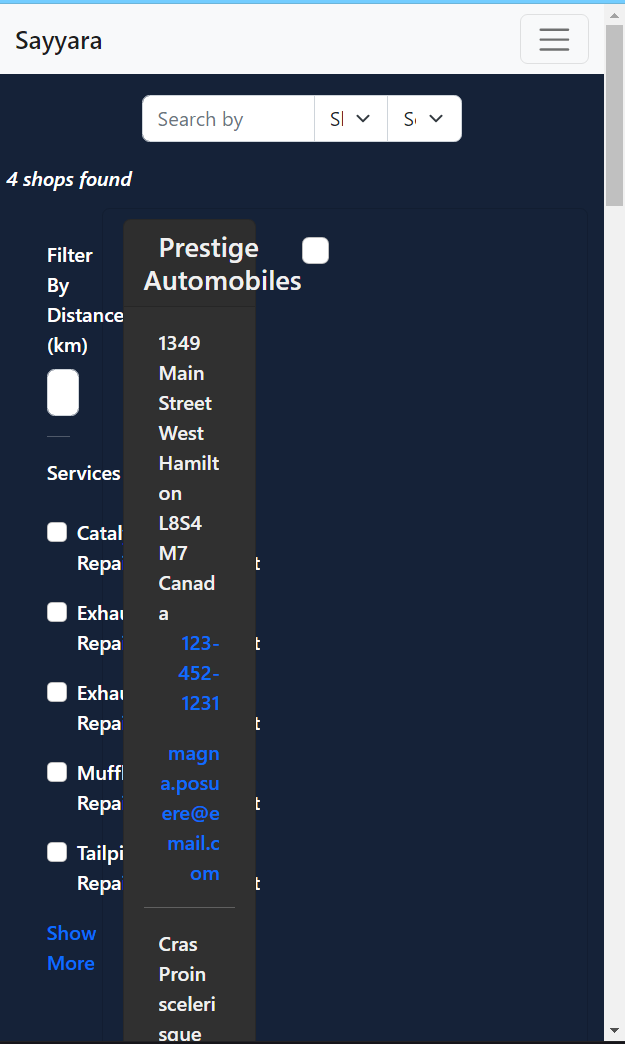
\includegraphics[width=0.50\textwidth]{VnVReport/result_images/mc_shoplookup.png}
%     \caption{MC-1: Shop Lookup feature when viewed on a reduced screen resolution}
%     \label{fig:mc_shoplookup}
% \end{figure}
% The issue with this feature is that the shop cards overlap other components on the page, and are stretched so the information in them is difficult to read by the user.

% \begin{figure}[H]
%     \centering
%     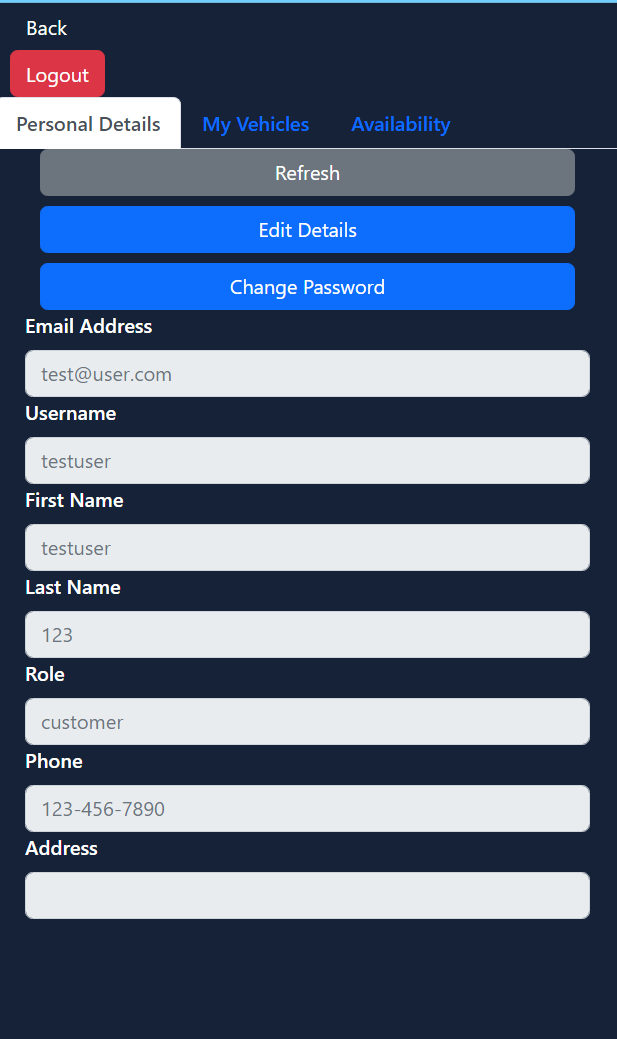
\includegraphics[width=0.50\textwidth]{VnVReport/result_images/mc_profile.png}
%     \caption{MC-2: User Profile feature when viewed on a reduced screen resolution}
%     \label{fig:mc_profile}
% \end{figure}
% The issue with this feature is the cluttered buttons and tabs at the top of the screen. These could be reorganized to prevent this from occurring.

% \begin{figure}[H]
%     \centering
%     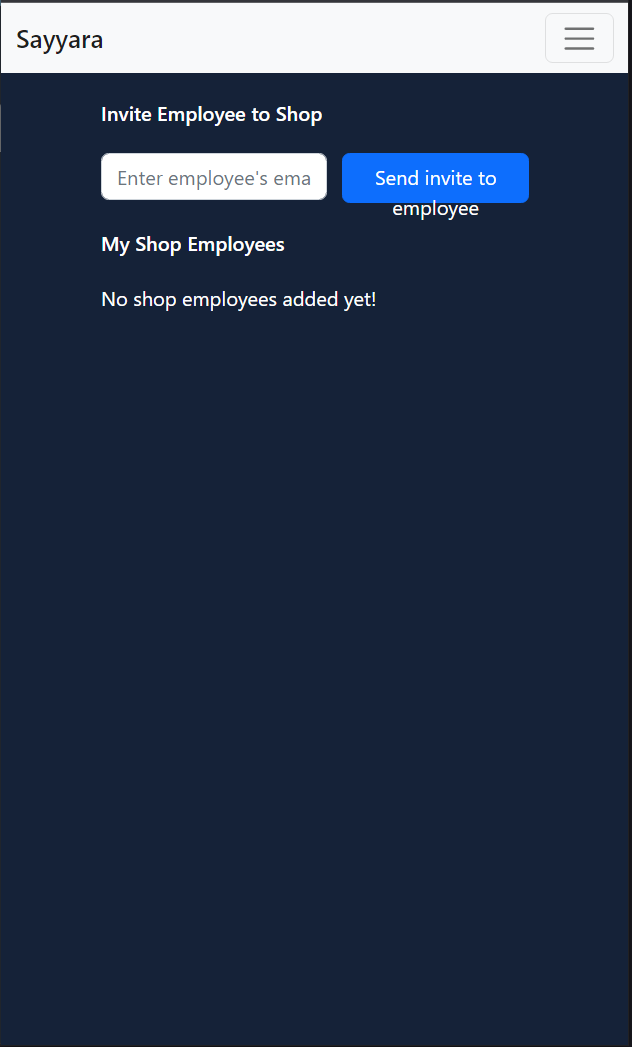
\includegraphics[width=0.50\textwidth]{VnVReport/result_images/mc_shop.png}
%     \caption{MC-3: Shop Employee Dashboard feature when viewed on a reduced screen resolution}
%     \label{fig:mc_shop}
% \end{figure}
% The issue with this feature is the textbox and button text is cut off due to the reduced screen resolution.

\subsection{Security}
    \subsubsection{Password Encryption}
        References requirement SR1\\
        Django uses PBKDF2 with SHA56 to hash the passwords when creating a user account. Taking a look at the database entries, we can see that the stored passwords are indeed encrypted and not stored as plain text. An example taken from the database can be seen in the figure below.

    \begin{table}[H]
        \centering
        \begin{tabularx}{\textwidth}{|c|p{2.3cm}|p{2.4cm}|p{2.5cm}|p{2.2cm}|p{2cm}|}
            \hline
            Id & Reference Requirement & User Action & Expected Results & Actual Result & Pass/Fail\\ \hline
            SR1-1 & SR1 & Create a test account and check database entry for the value stored in the password field & Encrypted password & Encrypted password & \textcolor{green}{Pass} \\ \hline
        \end{tabularx}
        \caption{Encryption test}
        %\label{tab:my_label}
    \end{table}
    
    \begin{figure}[H]
        \centering
        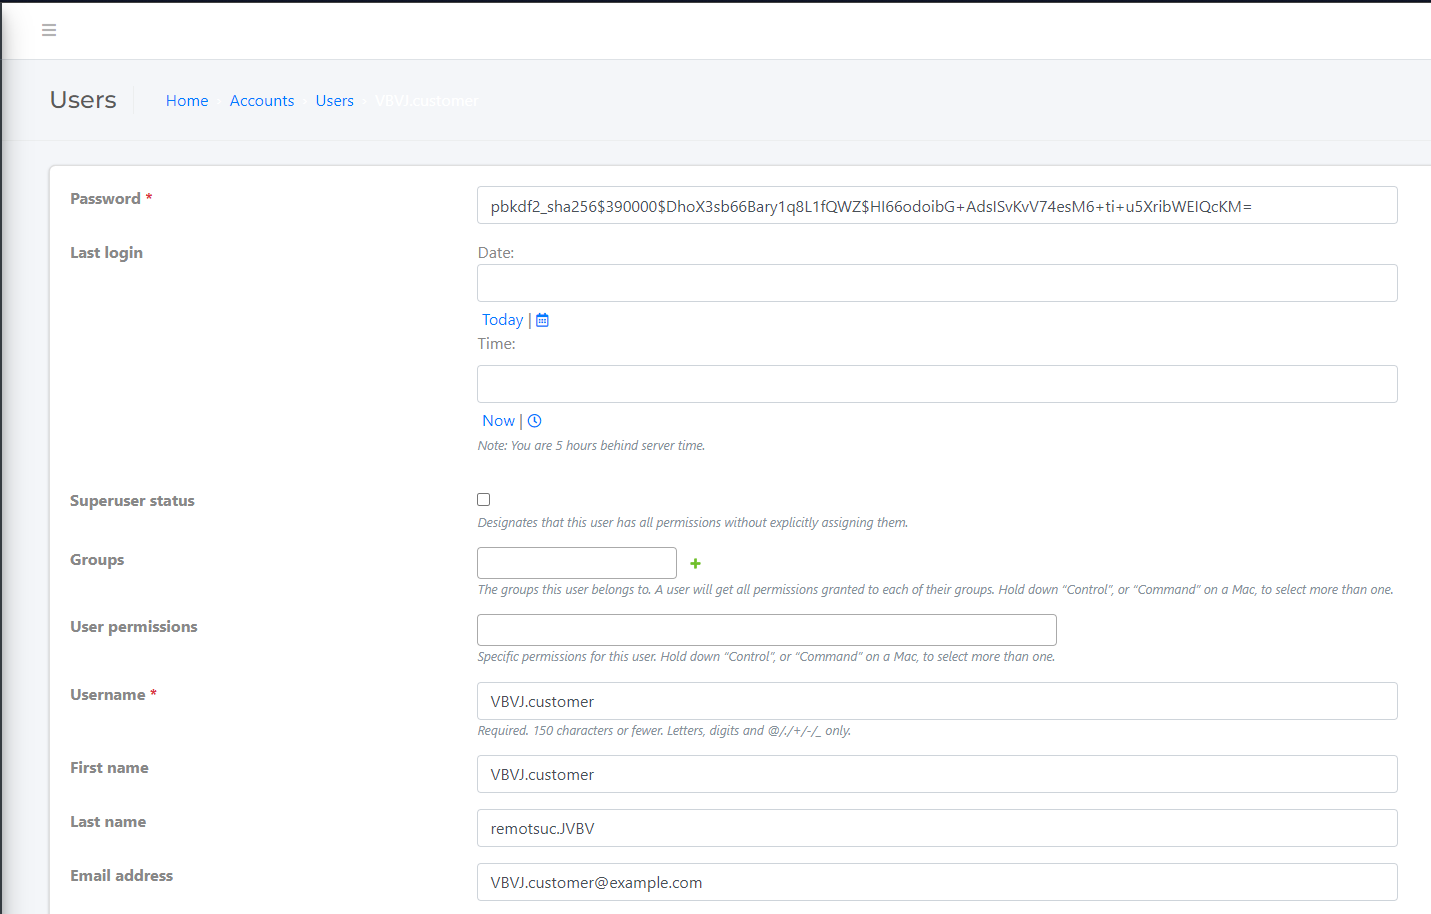
\includegraphics[width=1.1\textwidth]{VnVReport/result_images/password.png}
        \caption{How a user's password is stored within the database.}
        \label{fig:encryption}
    \end{figure}

    \subsubsection{Securing Personal Information}
        References requirement SR2\\
        This test is passed by default as the system does not even allow a user other than the one who created the data node (shop, appointment, etc) to perform any CRUD operations on it whatsoever.
    \subsubsection{Rate limiting}
        References requirement SR3\\
        Rate limiting database operations was beyond the scope of the system, and this this test (and its corresponding NFR) is not considered nor performed.

\subsection{Cultural and Political}
    \subsubsection{Offensive language}
        References requirement CPR1\\
        There was no trace of any potentially offensive language or profanity to be found within the source code of the project. This was verified by using the search for words function of VSCode and with a list of known offesnvie language.
    \subsubsection{Other languages}
        References requirement CPR2\\
        Supporting languages other than English was beyond the scope of the system, and this this test (and its corresponding NFR) is not considered nor performed.
    \subsubsection{Profanity filter for chat}
        References requirement CPR3\\
        This feature was not implemented yet and so validating this non functional requirement will come at a later time.

\subsection{Compliance}
    \subsubsection{Disclaimer upon registration and survey results}
        References requirement CR1\\
        As there is not a yet an end user agreement, disclaimer, etc. The test and survey that corresponds with this NFR could not be completed yet. The test and survey will have to be revisited at a later date when a disclaimer is created or provided by the primary stakeholder.

\section{Unit Testing}

The following test cases outline the unit tests in simple language. Please do note that the tests are implemented through a combination of backend unit tests.

\subsection{Register a new customer}
    \subsubsection{Module}
    \textbf{Customer}
    \subsubsection{Initial State}
    User fills out the registration form and submits the data
    \subsubsection{Results}
    A new customer is created with the provided data

\subsection{Sign in as customer}
    \subsubsection{Module}
    \textbf{Customer}
    \subsubsection{Initial State}
    User fills out the sign-in form and submits the data
    \subsubsection{Results}
    User is authenticated with the provided data

\subsection{Search for customers}
    \subsubsection{Module}
    \textbf{Customer}
    \subsubsection{Initial State}
    A \textbf{non-customer} is searching for customers
    \subsubsection{Results}
    A customer is found by the provided criteria

\subsection{View customer profile}
    \subsubsection{Module}
    \textbf{Customer}
    \subsubsection{Initial State}
    A customer has navigated to their profile
    \subsubsection{Results}
    The customer sees the relevant data pertaining to their account

\subsection{Edit customer profile}
    \subsubsection{Module}
    \textbf{Customer}
    \subsubsection{Initial State}
    A customer is editing their profile information
    \subsubsection{Results}
    The customer's profile information is updated

\subsection{Register a new employee}
    \subsubsection{Module}
    \textbf{Employee}
    \subsubsection{Initial State}
    The shop owner has already sent an invite for the user.
    User fills out the registration form and submits the data
    \subsubsection{Results}
    A new employee is created with the provided data

\subsection{Sign in as employee}
    \subsubsection{Module}
    \textbf{Employee}
    \subsubsection{Initial State}
    User fills out the sign-in form and submits the data
    \subsubsection{Results}
    User is authenticated with the provided data

\subsection{Search for employees}
    \subsubsection{Module}
    \textbf{Employee}
    \subsubsection{Initial State}
    An employee is searching for other employees
    \subsubsection{Results}
    An employee is found by the provided criteria

\subsection{View employee profile}
    \subsubsection{Module}
    \textbf{Employee}
    \subsubsection{Initial State}
    An employee has navigated to their profile
    \subsubsection{Results}
    The employee sees the relevant data pertaining to their account

\subsection{Edit employee profile}
    \subsubsection{Module}
    \textbf{Employee}
    \subsubsection{Initial State}
    An employee is editing their profile information
    \subsubsection{Results}
    The employee's profile information is updated

\subsection{Delete employee profile}
    \subsubsection{Module}
    \textbf{Employee}
    \subsubsection{Initial State}
    A shop owner is deleting an employee's profile ie, removing them from the shop.
    \subsubsection{Results}
    The employee profile is deleted from the database

\subsection{Register a new shop}
    \subsubsection{Module}
    \textbf{Shop}
    \subsubsection{Initial State}
    User fills out the registration form and submits the data after signing up as a shop owner.
    \subsubsection{Results}
    A new shop is created with the provided data

\subsection{Sign in as shop}
    \subsubsection{Module}
    \textbf{Shop}
    \subsubsection{Initial State}
    User fills out the sign-in form and submits the data as a shop owner
    \subsubsection{Results}
    User is authenticated with the provided data

\subsection{Search for shops}
    \subsubsection{Module}
    \textbf{Shop}
    \subsubsection{Initial State}
    A customer is searching for shops in their area
    \subsubsection{Results}
    A shop is found by the provided criteria

\subsection{View shop profile}
    \subsubsection{Module}
    \textbf{Shop}
    \subsubsection{Initial State}
    A customer has navigated to a shop's profile
    \subsubsection{Results}
    The customer sees the relevant data pertaining to the shop

\subsection{Edit shop profile}
    \subsubsection{Module}
    \textbf{Shop}
    \subsubsection{Initial State}
    A shop is editing their profile information
    \subsubsection{Results}
    The shop's profile information is updated

\subsection{Delete shop profile}
    \subsubsection{Module}
    \textbf{Shop}
    \subsubsection{Initial State}
    A shop is deleting their profile
    \subsubsection{Results}
    The shop profile is deleted from the database

\subsection{Add an employee to a shop}
    \subsubsection{Module}
    \textbf{Shop}
    \subsubsection{Initial State}
    A shop is adding an employee to their shop
    \subsubsection{Results}
    An employee is added to the shop

\subsection{Remove an employee from a shop}
    \subsubsection{Module}
    \textbf{Shop}
    \subsubsection{Initial State}
    A shop is removing an employee from their shop
    \subsubsection{Results}
    An employee is removed from the shop

\subsection{Add a service to a shop}
    \subsubsection{Module}
    \textbf{Shop}
    \subsubsection{Initial State}
    A shop is adding a service to their shop
    \subsubsection{Results}
    A service is added to the shop

\subsection{Remove a service from a shop}
    \subsubsection{Module}
    \textbf{Shop}
    \subsubsection{Initial State}
    A shop is removing a service from their shop
    \subsubsection{Results}
    A service is removed from the shop

\subsection{Add a vehicle to a customer's profile}
    \subsubsection{Module}
    \textbf{Vehicle}
    \subsubsection{Initial State}
    A customer is adding a vehicle to their profile
    \subsubsection{Results}
    A vehicle is added to the customer profile

\subsection{Remove a vehicle from a customer's profile}
    \subsubsection{Module}
    \textbf{Vehicle}
    \subsubsection{Initial State}
    A customer is removing a vehicle from their profile
    \subsubsection{Results}
    A vehicle is removed from the customer profile

\subsection{Add an appointment to a shop}
    \subsubsection{Module}
    \textbf{Appointment}
    \subsubsection{Initial State}
    A shop is adding an appointment to their schedule
    \subsubsection{Results}
    An appointment is added to the shop schedule

\subsection{Remove an appointment from a shop}
    \subsubsection{Module}
    \textbf{Appointment}
    \subsubsection{Initial State}
    A shop is removing an appointment from their schedule
    \subsubsection{Results}
    An appointment is removed from the shop schedule

\subsection{Add an availability to an employee}
    \subsubsection{Module}
    \textbf{Availability}
    \subsubsection{Initial State}
    An employee is adding an availability to their schedule
    \subsubsection{Results}
    An availability is added to the employee schedule

\subsection{Remove an availability from an employee}
    \subsubsection{Module}
    \textbf{Availability}
    \subsubsection{Initial State}
    An employee is removing an availability from their schedule
    \subsubsection{Results}
    An availability is removed from the employee schedule

\subsection{Create a work order}
    \subsubsection{Module}
    \textbf{Work order}
    \subsubsection{Initial State}
    A customer is creating a work order
    \subsubsection{Results}
    A work order is created

\subsection{Edit a work order}
    \subsubsection{Module}
    \textbf{Work order}
    \subsubsection{Initial State}
    A customer is editing a work order
    \subsubsection{Results}
    A work order is updated

\subsection{Delete a work order}
    \subsubsection{Module}
    \textbf{Work order}
    \subsubsection{Initial State}
    A customer is deleting a work order
    \subsubsection{Results}
    A work order is deleted from the database

\subsection{Add a service to a work order}
    \subsubsection{Module}
    \textbf{Work order}
    \subsubsection{Initial State}
    A customer is adding a service to a work order
    \subsubsection{Results}
    A service is added to the work order

\subsection{Remove a service from a work order}
    \subsubsection{Module}
    \textbf{Work order}
    \subsubsection{Initial State}
    A customer is removing a service from a work order
    \subsubsection{Results}
    A service is removed from the work order

\subsection{Add an employee to a work order}
    \subsubsection{Module}
    \textbf{Work order}
    \subsubsection{Initial State}
    A customer is adding an employee to a work order
    \subsubsection{Results}
    An employee is added to the work order

\subsection{Remove an employee from a work order}
    \subsubsection{Module}
    \textbf{Work order}
    \subsubsection{Initial State}
    A customer is removing an employee from a work order
    \subsubsection{Results}
    An employee is removed from the work order

\subsection{Create a conversation}
    \subsubsection{Module}
    \textbf{Conversation}
    \subsubsection{Initial State}
    A customer is creating a conversation
    \subsubsection{Results}
    A conversation is created

\subsection{Edit a message}
    \subsubsection{Module}
    \textbf{Conversation}
    \subsubsection{Initial State}
    A customer is editing a message
    \subsubsection{Results}
    A conversation is updated

\subsection{Search for a shop by name}
    \subsubsection{Module}
    \textbf{Shop Lookup}
    \subsubsection{Initial State}
    A customer is searching for a shop 
    \subsubsection{Results}
    A list of all shops names that contain the query is provided

\subsection{Search for a shop by address}
    \subsubsection{Module}
    \textbf{Shop Lookup}
    \subsubsection{Initial State}
    A customer is searching for a shop 
    \subsubsection{Results}
    A list of all shops addresses that match the query is provided

\subsection{Filter shops by services}
    \subsubsection{Module}
    \textbf{Shop Lookup}
    \subsubsection{Initial State}
    A customer is provides a list of desired services
    \subsubsection{Results}
    A list of all shops that provide the service is provided

\subsection{Filter shops by distance}
    \subsubsection{Module}
    \textbf{Shop Lookup}
    \subsubsection{Initial State}
    A customer is filtering shops that are further than a certain distance in km
    \subsubsection{Results}
    A list of all shops names are no further than the specified distance is provided

\subsection{Sort shops by name}
    \subsubsection{Module}
    \textbf{Shop Lookup}
    \subsubsection{Initial State}
    A customer is sorting search results alphabetically 
    \subsubsection{Results}
    A list of shops that match the filter and search ordered alphabetically (or in reverse)

\subsection{Sort shops by distance}
    \subsubsection{Module}
    \textbf{Shop Lookup}
    \subsubsection{Initial State}
    A customer is sorting search results from closest to furthest
    \subsubsection{Results}
    A list of shops that match the filter and search ordered by distance (or in reverse)


\section{Changes Due to Testing}

Several initial test failures revealed unimplemented functional requirements such as the lack of password format validity checking. Others exposed bugs including the profile update backend failing to save phone number changes. These missing features and bugs were then implemented and resolved, respectively. Frontend testing revealed an additional bug involving the profile update page failing silently, which will be addressed prior to the next revision.

Performing some of the nonfunctional tests that had to do with compatibility on both web and mobile highlighted some visual issues that 
will need to be addressed in the next iteration of the application. Additionally, performing the database efficiency testing highlighted 
that more visual indicators need to be implemented so the user realizes that the page is loading and is still responding. Overall, from 
nonfunctional testing and stakeholder feedback, there needs to be some visual improvements implemented to ensure the user has the best 
possible experience while using the Sayyara application.

\section{Automated Testing}

\subsection{System Uptime Stress Testing}
% As mentioned in section 6.2.1, the stress testing of the system will be performed using an automated testing tool such as JMeter once deployment is completed.

As of revision 1 of the project, the application does not need to be deployed as per our project supervisor Nabil. System uptime stress testing will no longer be required for this revision.

\subsection{Unit Testing}

As mentioned in section 8, the unit testing is managed by automated tests writing in Python and Javascript for automating the given test scenarios.

\begin{figure}[H]
    \centering
    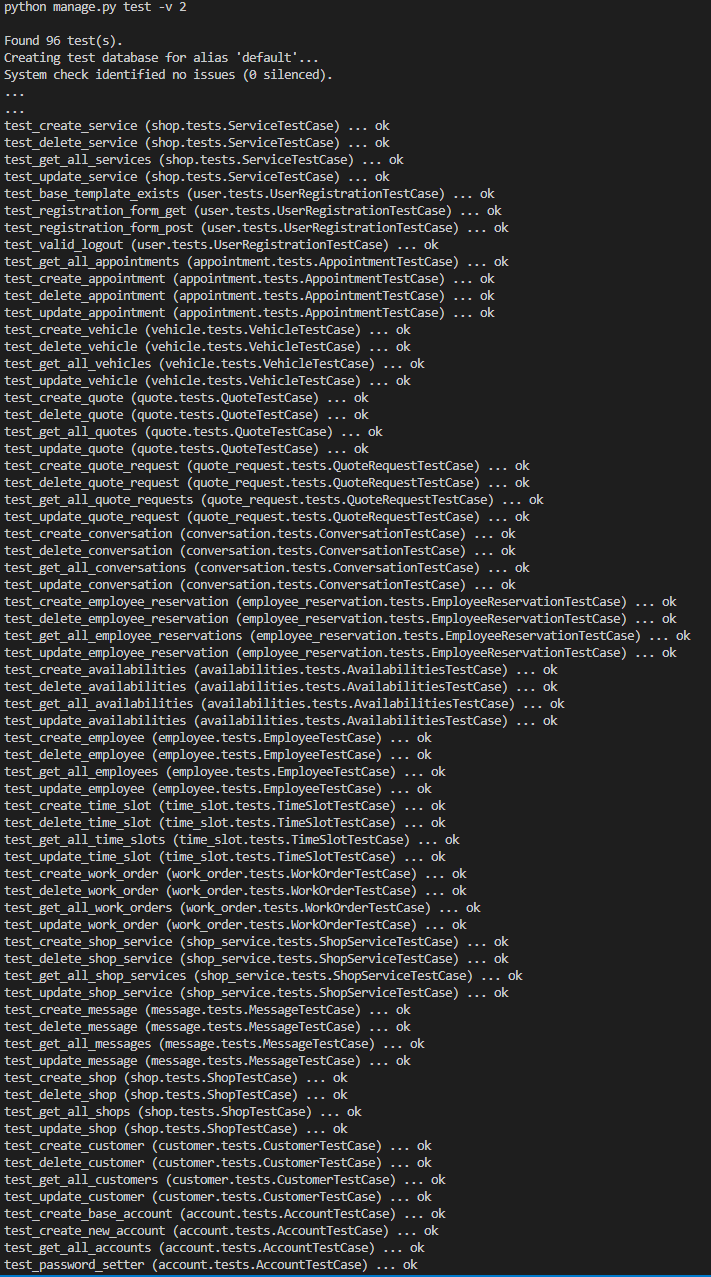
\includegraphics[width=0.80\textwidth]{VnVReport/result_images/unit-tests.png}
    \caption{Unit Tests run using pytest through Django framework}
    \label{fig:unit-testing}
\end{figure}

\subsection{End-To-End Testing}

Also known as user acceptance testing or E2E testing is also deployed in an automated environment simulating different user agents and user-scenarios to further validate and verify functional requirements down to the user-interface level. The following is a subset of all the E2E tests that cover the requirements given. Note that the steps are implemented in code using javascript and the playwright framework.

\begin{itemize}
    \item \textbf{Customer Module}
    \begin{enumerate}
        \item A user can register as a customer on the web app.
        \begin{itemize}
            \item Select the "Sign up" button
            \item Fill out the form to create the account
            \item Confirm your email by clicking the link sent by email.
            \item Log in using the credentials.
        \end{itemize}
        \item A user can create a quote request.
        \begin{itemize}
            \item Log in as a customer.
            \item Select the "Post a quote request" button.
            \item Fill out the form.
            \item Click "Save".
        \end{itemize}
        \item A user can create a vehicle.
        \begin{itemize}
            \item Log in as a customer.
            \item Select the "Profile" tab.
            \item Select the "New Vehicle" button.
            \item Fill out the form.
            \item Click "Create".
        \end{itemize}
    \end{enumerate}
    \item \textbf{Shop Owner Module}
    \begin{enumerate}
        \item A user can register as a shop owner on the web app.
        \begin{itemize}
            \item Select the "Sign up" button
            \item Fill out the form to create the account
            \item Confirm your email by clicking the link sent by email.
            \item Log in using the credentials.
        \end{itemize}
        \item A user can create a shop on the web app.
        \begin{itemize}
            \item Log in as a shop owner.
            \item Select the "Shops" tab.
            \item Select the "New Shop" button.
            \item Fill out the form.
            \item Click "Create".
        \end{itemize}
        \item A user can create an appointment on the web app.
        \begin{itemize}
            \item Log in as a shop owner.
            \item Select the "Shops" tab.
            \item Select the "New Appointment" button.
            \item Fill out the form.
            \item Click "Save".
        \end{itemize}
        \item A user can create a quote on the web app.
        \begin{itemize}
            \item Log in as a shop owner.
            \item Select the "Shops" tab.
            \item Select the "New Quote" button.
            \item Fill out the form.
            \item Click "Create".
        \end{itemize}
    \end{enumerate}
    \item \textbf{Employee Module}
    \begin{enumerate}
        \item A user can register as a shop employee on the web app.
        \begin{itemize}
            \item Select the "Sign up" button
            \item Fill out the form to create the account
            \item Confirm your email by clicking the link sent by email.
            \item Log in using the credentials.
        \end{itemize}
        \item A user can create a shop employee reservation on the web app.
        \begin{itemize}
            \item Log in as a shop employee.
            \item Select the "Shops" tab.
            \item Select the "New Shop Employee Reservation" button.
            \item Fill out the form.
            \item Click "Save".
        \end{itemize}
    \end{enumerate}
        \item \textbf{Messaging Module}
    \begin{enumerate}
        \item A user can message other users using the web app.
        \begin{itemize}
            \item Log in as a customer.
            \item Select the "Conversations" tab.
            \item Select the "New Conversation" button.
            \item Fill out the form.
            \item Click "Create".
            \item The message should be received.
        \end{itemize}
    \end{enumerate}
    \item \textbf{Shop Search Module}
    \begin{enumerate}
        \item A user can search the web app for shops based on location.
        \begin{itemize}
            \item Log in as a customer.
            \item Enter a location in the "Search" field.
            \item Shops matching the search should be displayed.
        \end{itemize}
    \end{enumerate}
    \item \textbf{Quotes Module}
    \begin{enumerate}
        \item A user can post a quote request on the web app.
        \begin{itemize}
            \item Log in as a customer.
            \item Select the "Quote requests" tab.
            \item Select the "New Quote request" button.
            \item Fill out the form.
            \item Click "Create".
        \end{itemize}
        \item A user can post a quote on the web app.
        \begin{itemize}
            \item Log in as a shop owner.
            \item Select the "Quote requests" tab.
            \item Select the "New Quote" button.
            \item Fill out the form.
            \item Click "Create".
        \end{itemize}
    \end{enumerate}
     \item \textbf{Reservations Module}
    \begin{enumerate}
        \item A user can create a reservation on the web app.
        \begin{itemize}
            \item Log in as a customer.
            \item Select the "Shops" tab.
            \item Select the "New Reservation" button.
            \item Fill out the form.
            \item Click "Save".
        \end{itemize}
        \item A user can create a shop employee reservation on the web app.
        \begin{itemize}
            \item Log in as a shop employee.
            \item Select the "Shops" tab.
            \item Select the "New Shop Employee Reservation" button.
            \item Fill out the form.
            \item Click "Save".
        \end{itemize}
    \end{enumerate}
    \item \textbf{Shops Module}
    \begin{enumerate}
        \item A user can create a shop on the web app.
        \begin{itemize}
            \item Log in as a shop owner.
            \item Select the "Shops" tab.
            \item Select the "New Shop" button.
            \item Fill out the form.
            \item Click "Create".
        \end{itemize}
    \end{enumerate}
    \item \textbf{Vehicles Module}
    \begin{enumerate}
        \item A user can create a vehicle on the web app.
        \begin{itemize}
            \item Log in as a customer.
            \item Select the "Vehicles" tab.
            \item Select the "New Vehicle" button.
            \item Fill out the form.
            \item Click "Save".
        \end{itemize}
    \end{enumerate}
    \item \textbf{Work Orders Module}
    \begin{enumerate}
        \item A user can create a work order on the web app.
        \begin{itemize}
            \item Log in as a customer.
            \item Select the "Work Orders" tab.
            \item Select the "New Work Order" button.
            \item Fill out the form.
            \item Click "Create".
        \end{itemize}
    \end{enumerate}
    \item \textbf{Appointments Module}
    \begin{enumerate}
        \item A user can create an appointment on the web app.
        \begin{itemize}
            \item Log in as a shop owner.
            \item Select the "Appointments" tab.
            \item Select the "New Appointment" button.
            \item Fill out the form.
            \item Click "Save".
        \end{itemize}
    \end{enumerate}
\end{itemize}


\newpage
\section{Trace to Requirements}

    \begin{table}[H]
        \centering
        \begin{tabularx}{\textwidth}{|c|X|c|X|}
            \hline
            \textbf{FR} & \textbf{Tests} & \textbf{FR} & \textbf{Tests} \\ \hline
            AuR1 & FR-AR1-1, FR-AR1-2, FR-AR1-3 & AuR2 & FR-AR2-1, FR-AR2-2A, FR-AR2-2B \\ \hline
            AuR3 & FR-AR2-3 & SR1 & \\ \hline
            SR2 & & SR3 & \\ \hline
            PAR1 & & PAR2 & \\ \hline
            PAR3 & FR-PAR3-1, FR-PAR3-2 & PAR4 & \\ \hline
            PAR5 & FR-VE1-1.1, FR-VE1-1.2, FR-VE1-1.3, FR-VE1-1.4 & PAR6 & \\ \hline
            PAR7 & & PAR8 & \\ \hline
            PAR9 & & PAR10 & \\ \hline
            PAR11 & & ApR1 & FR-APR1-1.1 \\ \hline
            ApR2 & FR-ARP2-1.1 & ApR3 & FR-APR3-1.1 \\ \hline
            ApR4 & FR-APR4-1.1 & ApR5 & FR-APR5-1.1 \\ \hline
            WOR1 & & WOR2 & \\ \hline
            WOR3 & & QR1 & FR-QR1-1.1, FR-QR1-1.2 \\ \hline
            QR2 & FR-QR2-1.1, FR-QR2-1.2, FR-QR2-1.3 & QR3 & FR-QR2-1.1, FR-QR2-1.2, FR-QR2-1.3 \\ \hline
 %           VR1 & & VR2 & \\ \hline
        \end{tabularx}
        \caption{Traceability between Tests and Functional Requirements}
        \label{tab:frtrace}
    \end{table}

    \begin{table}[H]
        \centering
        \begin{tabularx}{\textwidth}{|c|X|c|X|}
            \hline
            \textbf{NFR} & \textbf{Tests} & \textbf{NFR} & \textbf{Tests} \\ \hline
            LFR1 & NFR-LFR1-1 & LFR2 & NFR-LFR2-1 \\ \hline
            LFR3 & NFR-LFR3-1 & LFR4 & NFR-LFR4-1 \\ \hline
            LFR5 & NFR-LFR5-1 & UHR1 & NFR-UHR1-1, NFR-UHR1-2 \\ \hline
            UHR2 & NFR-UHR2-1 & UHR3 & NFR-UHR3-1 \\ \hline
            UHR4 & NFR-UHR4-1 & UHR5 & NFR-UHR5-1 \\ \hline
            PR1 & NFR-PR1-1 & PR2 & SSU-1 \\ \hline
            PR3 & DE-1, DE-2, DE-3 & OER1 & IBC-1, IBC-2, IBC-3, IBC-4 \\ \hline
            % OER2 & MC-1, MC-2, MC-3 & OER3 & \\ \hline
            MSR1 & & & \\ \hline
            SR1 & Section 6.5.1 & SR2 & Section 6.5.2 \\ \hline
            SR3 & Section 6.5.3 & CPR1 & Section 6.6.1 \\ \hline
            CPR2 & Section 6.6.2 & CPR3 & Section 6.6.3 \\ \hline
            CR1 & Section 6.7.1 & & \\ \hline
        \end{tabularx}
        \caption{Traceability between Tests and Non-functional requirements}
        \label{tab:nfrtrace}
    \end{table}

\newpage
\section{Trace to Modules}

    \begin{table}[H]
        \centering
        \begin{tabularx}{\textwidth}{|c|X|c|X|}
            \hline
            \textbf{Module} & \textbf{Tests} & \textbf{Module} & \textbf{Tests} \\ \hline
            FE1 & FR-AR2-1, FR-AR2-2A, FR-AR2-2B & BE1 & FR-AR1-1, FR-AR1-2, FR-AR1-3, FR-PAR3-1, FR-PAR3-2 \\ \hline
            FE2 & FR-VE1-1.1 & BE2 & FR-VE1-1.2, FR-VE1-1.3, FR-VE1-1.4 \\ \hline
            FE3 & NFR-LFR1-1, NFR-UHR1-1 & BE3 & FR-AP1-1.1, FR-AP2-1.1 \\ \hline
            FE4 & & BE4 & FR-AP1-1.1, FR-AP2-1.1 \\ \hline
            FE5 & & BE5 & N/A \\ \hline
            FE6 & NFR-LFR1-1 & BE6 & FR-AP1-1.1, FR-AP2-1.1 \\ \hline
            FE7 & NFR-LFR1-1 & BE7 & FR-VE1-1.1, FR-VE1-1.2 \\ \hline
            FE8 & NFR-LFR1-1 & BE8 & FR-QR1-1.1, FR-QR1-1.2, FR-QR2-1.1, FR-QR2-1.2 \\ \hline
            FE9 & FR-QR1-1.1, FR-QR2-1.1, FR-QR2-1.2, FR-QR2-1.3 & BE9 & FR-QR1-1.1, FR-QR2-1.1\\ \hline
            FE10 & FR-QR1-1.2, FR-QR2-1.2, FR-QR2-1.3 & BE10 & FR-AP2-1.1, FR-AP4-1.1 \\ \hline
            FE11 & & BE11 & N/A \\ \hline
            FE12 & N/A & & \\ \hline
            FE13 & FR-AP1-1.1, FR-AP2-1.1, FR-AP4-1.1 & & \\ \hline
            FE14 & & & \\ \hline
        \end{tabularx}
        \caption{Traceability between Tests and Modules}
        \label{tab:modtrace}
    \end{table}

\section{Code Coverage Metrics}

\begin{figure}[H]
    \centering
    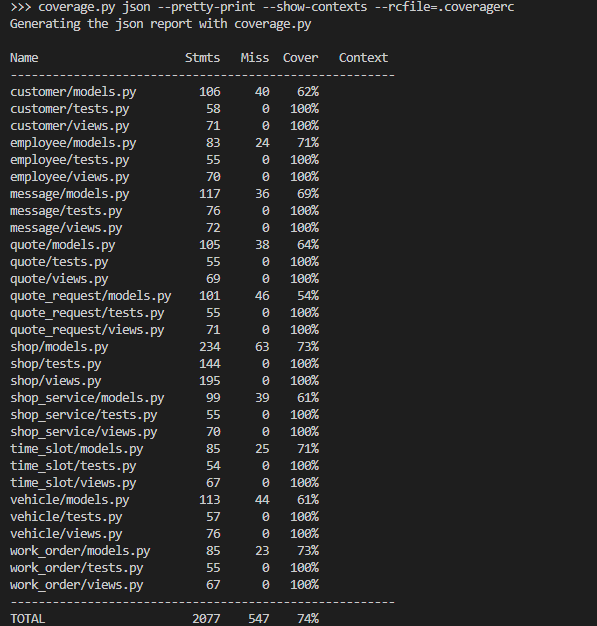
\includegraphics[width=0.80\textwidth]{VnVReport/result_images/coverage.png}
    \caption{Code coverage of the backend using coverage.py}
    \label{fig:unit-testing}
\end{figure}

\bibliographystyle{plainnat}
\bibliography{../../refs/References}

\newpage{}
\section*{Appendix --- Reflection}

The information in this section will be used to evaluate the team members on the
graduate attribute of Reflection.  Please answer the following question:

\begin{enumerate}
  \item In what ways was the Verification and Validation (VnV) Plan different
  from the activities that were actually conducted for VnV?  If there were
  differences, what changes required the modification in the plan?  Why did
  these changes occur?  Would you be able to anticipate these changes in future
  projects?  If there weren't any differences, how was your team able to clearly
  predict a feasible amount of effort and the right tasks needed to build the
  evidence that demonstrates the required quality?  (It is expected that most
  teams will have had to deviate from their original VnV Plan.)
\end{enumerate}

Reflections

\begin{itemize}
    \item Harsh: The VnV Plan for the Sayyara project stayed similar to the activities that were actually conducted for VnV, with the exception of the scope of user testing. The changes to the original VnV Plan came about in response to feedback from stakeholders, which indicated that the user interface was not as intuitive or user-friendly as desired. In future projects, it may be possible to anticipate the need to adjust the scope of VnV activities, depending on the nature of the product and feedback from stakeholders.

    \item Alyssa: In terms of the nonfunctional requirement testing, for the most part, the VnV Plan stayed the same. What changed were some of the methods of testing these requirements. For example, for database efficiency testing, when writing the VnV Plan, it was undetermined what would be used to test this. After doing research while testing, I was able to find a dedicated profiling tool for Django that performed the exact tests I needed for the VnV Report. This change occurred because I was looking for a simple but effective solution that was catered to the exact framework we are using for the backend. Otherwise, I would've had to have spend time manually querying database entries and writing debug messages to determine how long they took. Changes in future projects would depend on the requirements of the project, as well as feedback from stakeholders on whether or not this type of VnV would be necessary to ensure the product meets the requirements.

    \item Collin: For the most part, the VnV Plan was quite similar to the activites that were ultimately performed. However, there were a few differences between the VnV Plan and the activities that were actually conducted. For some non function requirements testing, namely the compliance and security, and political ones, the test plans that were proposed were either unnecessary, did not need to be automated (i.e. manually testing would have sufficed), was beyond the scope of what is reasonable given the time frame, or the features were simply not implemented. This resulted in the initial VnV plan requiring more work and effort than required and would not really improve the validation an verification of the system, so changes to the some of the testing methods had to be made. In future projects, changes to non-functional requirements VnV could possibly be anticipated, as the scope of the project can always change, some features deemed unnecessary or unneeded.

    \item Chris: The VnV Plan and VnV Report are not much different, except a few key areas. Firstly, some new testing frameworks were added to the frontend to better facilitate user interaction testing. These frameworks were not considered before, because at the time of the VnV Plan creation, development was still in its beginning stages, and as such there was not much yet to test; much of it was anticipation of modules and planning. However, after creating the user interface, the team noticed a need for a tool that can more quickly test clicks and interactions on the website. Additionally, there were some changes to non-functional requirement testing methodologies. For example, test NFR-LR1-1 was planned to be executed by using a tool that can visualize an interaction tree, but no such framework could be found in time that was compatible with our project. This was a mistake on my part, as I should have done more research to verify if conducting such a test was even possible. Overall, the changes made were mostly in pursuit of finding more efficient and easier methods of testing. These changes could've been anticipated if more research was done on testing frameworks, and if some practice tests were written first to gauge the difficulty in writing them, or if we sought out more experienced advice. As someone who hasn't done much test development, it was a vital learning experience for me, learning the importance of research, efficient tools, and not underestimating the difficulty of testing scope. Most of the rest of the VnV Plan was accurate, due to the team's experience with some of the initial testing frameworks we chose, as well as due to the team's concrete planning of what all the modules will be and how they would precisely interact.

    \item Kai: The VnV plan was devised prior to the design documents and most of the implementation, and as such did not have as much specific details on test cases and specific features to test for, compared to those outlined in the VnV report. A major source of deviation was the relatively large breadth of the features in the application, and the uncertainties in the depth for the implementation of each. Ideally, the implementation should follow the SRS as closely as possible, and so the VnV should readily verify the SRS regardless of implementation details. In practice, due to time constraints and uneven familiarity with some of the tech stacks, changes were made to facilitate rapid implementation that cover as much of the requirement as possible. In spite of the differences, following rev0 implementations we were able to devise more time-feasible test cases with a small number of both success and failure scenarios for each major requirement, both manual and automatic, for the frontend and the backend, as documented in the VnV report. The deviations served as a good example of what to expect in the future, and highlights the advantages of a test-driven development process, in which tests and development can be coupled more closely.

    \item Ethan: There are two main differences I see between the VnV plan and the actual VnV work that took place:
        \begin{enumerate}
            \item The number of tests planned was much lower than the number of tests performed. The VnV plan does a decent job of outlining the broad categories of tests which need to be performed, but within each of those categories is around 2-4 individual tests that need to be run: at least one for both normal and abnormal inputs, in addition to any boundary values. This change should be quite easy to anticipate in future projects as these types of test cases are quite commonly used.
            \item The control method of most frontend testing was manual, while the backend was mostly automatic. This change was made as the team discovered that manually testing the frontend portions of the system was much more time efficient than writing automatic tests, whereas the backend was much easier to automate. Running frontend manual tests allows for checking many aspects of the design at once such as errors rendering, layout problems, text formatting, color/contrast issues, etc. all in a much shorter time. Future projects might have a different approach to this problem (especially if the frontend framework or architecture is different), so anticipating which control method to use may still be difficult. Of course, this experience should mean more thought goes towards the problem next time.
        \end{enumerate}
\end{itemize}
\end{document}